\section{ Study of Neutrino Distribution using Conservation Laws}\label{ch:model_ind}

\subsection{Effective Number of Neutrinos}\label{sec:N_nu}
In the previous chapter we gave an overview of cosmology that included a simple model of neutrino freeze-out, wherein neutrinos decouple prior to the $e^\pm$ annihilation reheating period, leading to the reheating ratio in the decoupled limit \req{T_nu_T_gamma} which we now denote by $R_\nu$. However, as we mentioned several times this is only an approximate model. In reality, the freeze-out and reheating periods overlap to some degree which greatly complicates the picture, as some energy and entropy from the annihilating $e^\pm$ goes into neutrinos.  This overlap has observable consequences, as any extra energy in neutrinos impacts the speed of expansion of the Universe, through the Hubble equation \req{Hubble_eq}.

The additional energy and entropy fed into neutrinos is typically quantified by the effective number of neutrinos, $N_\nu$, defined by comparing the total neutrino energy density to the energy density of a massless fermion with two degrees of freedom and neutrino to photon temperature ratio $R_\nu$,
\begin{equation}
N_{\nu}=\frac{\rho_\nu}{\frac{7}{120}\pi^2  \left(R_\nu T_\gamma\right)^4}.
\end{equation}
 By definition, any transfer of energy from $e^\pm$ into neutrinos results in $N_\nu>N_\nu^f=3$, the number of physical neutrino flavors.  $N_\nu$ can be  measured by fitting to observational data, such as the Planck CMB measurements. A numerical computation based on the Boltzmann equation with two body scattering~\cite{Mangano2005} gives to $N_{\nu}^{\rm th}=3.046$. However the Planck CMB results contain several fits~\cite{Planck} based on different data sets which suggest that $N_\nu$ is in the range $3.30\pm 0.27$ to $3.62\pm0.25$ ($68\%$ confidence level). 

This tension between the Planck results and theoretical reheating studies motivates our work. This tension has inspired various theories, such as \cite{Weinberg:2013kea}, where it is postulated to be due to the presence of as yet undiscovered particle species. In this work, we avoid postulating the existence of additional particles, but rather explore the possibility that the increase in $N_\nu$ is the consequences of additional energy and entropy being transferred into neutrinos during $e^\pm$ annihilation.  In other words, we postulate additional neutrino reheating and explore its consequences.



\subsection{Matter Content}
In this work, matter will be modeled by a particle distribution function $f(t,x,p)$ that, roughly speaking, gives the probability of finding a particle per unit spacial volume per unit momentum space volume at a given time.  The distribution function gives the stress energy tensor, particle four-current, and entropy four-current via 
\begin{align}
T^{\mu,\nu}(t,x)=&\frac{g_p}{(2\pi)^3}\int p^\mu p^\nu f(t,x,p) \sqrt{|g|}\frac{d^3p}{p_0},\\
n^\nu(t,x)=&\frac{g_p}{(2\pi)^3}\int p^\nu f(t,x,p) \sqrt{|g|}\frac{d^3p}{p_0},\\
s^\nu(t,x)=&-\frac{g_p}{(2\pi)^3}\int(f\ln(f)\pm(1\mp f)\ln(1\mp f))p^\mu\sqrt{|g|}\frac{d^3p}{p_0}
\end{align}
where the upper signs are for fermions, the lower for bosons, $g_p$ is the degeneracy of the particle, and $g$ is the determinant of the metric.  In a flat FRW Universe, the expressions for the  energy density, pressure, number density, and entropy density of a particle of mass $m$ are
\begin{align}\label{moments}
\rho=&\frac{g_p}{(2\pi)^3}\int f(t,x,p)Ed^3p,\\
P=&\frac{g_p}{(2\pi)^3}\int f(t,x,p)\frac{p^2}{3E}d^3p,\\
n=&\frac{g_p}{(2\pi)^3}\int f(t,x,p) d^3p, \hspace{2mm} E=\sqrt{m^2+p^2},\\
s=&-\frac{g_p}{(2\pi)^3}\int (f\ln(f)\pm(1\mp f)\ln(1\mp f)) d^3p.
\end{align}

The dynamics of the distribution function,  and therefore the precise nature of neutrino freeze-out and the energy and entropy transferred into the neutrino sector, are governed by the Boltzmann equation
\begin{equation}
p^\alpha\partial_{x^\alpha} f-\Gamma^{j}_{\mu,\nu}p^\mu p^\nu\partial_{p^j}f=C[f]
\end{equation}
where repeated Greek indices indicate a sum over $0,...,3$ and Roman indices indicate a sum over the spacial components $1,...,3$.  The right hand side is the collision operator and incorporates the physics of any short range interactions that the particles participate in. The left hand side gives the dynamics under any long range forces. For us the only long range force will be gravity, encoded in the Christoffel symbols $\Gamma^j_{\mu\nu}$, and so the Boltzmann equation expresses the fact that particles undergo geodesic motion in between collisions. For much greater detail on the definition of the distribution function in a general spacetime, the geometric origin of the Boltzmann equation, and various properties and relations satisfied by moments of the distribution function, see for example \cite{andre,cercignani,bruhat,ehlers,kolb,bernstein2004kinetic}.

We will study neutrino freeze-out in detail using the Boltzmann equation in the second part of this dissertation, starting in chapter \ref{ch:boltz_orthopoly}. However, in this chapter we pursue a model independent approach wherein we assume instantaneous chemical/kinetic equilibrium and sharp freeze-out transitions between them.  Though limited in the kinds of questions we can address and answer, this approach makes up for these limitations by letting us derive several important properties that are independent of microscopic dynamics, i.e. independent of $C[f]$, so long as these assumptions are sufficiently accurate.  The dynamics will be derived from conservation laws involving the moments \ref{moments}, but first we must describe the distinction between chemical and kinetic equilibrium.


\subsubsection{Chemical and Kinetic Equilibrium}
%%%%%%%%%%%%%%%%%%%%%%%%%%%%%%%%%%%%
At sufficiently high temperatures, such as existed in the early Universe, both particle creation and annihilation (i.e. chemical) processes and momentum exchanging (i.e. kinetic) scattering processes can occur sufficiently rapidly to establish complete thermal equilibrium of a given particle species. The most probable canonical distribution function $f_{ch}^\pm$ of  fermions (+) and bosons (-) in both chemical and kinetic equilibrium is found by maximizing entropy subject to energy being conserved
\begin{equation}\label{ch_eq}
f_{ch}^\pm=\frac{1}{\exp(E/T)\pm 1}, \hspace{2mm} T>T_{ch}
\end{equation}
where $E$ is the particle energy, $T$ the temperature, and $T_{ch}$ the chemical freeze-out temperature. 


For a physical system comprising {\em interacting} particles whose temperature is decreasing with time, there will be a period where the temperature is greater than the kinetic freeze-out temperature, $T_k$, but below chemical freeze-out. During this period, momentum exchanging processes continue to maintain an equilibrium distribution of energy among the available particles, which we call kinetic equilibrium, but particle number changing processes no longer occur rapidly enough to keep the equilibrium particle number yield, i.e. for $T<T_{ch}$ the particle number changing processes have `frozen-out'. In this condition the momentum distribution, which is in kinetic equilibrium but chemical non-equilibrium, is obtained by maximizing  entropy subject to  particle number and energy constraints and thus two parameters appear
\begin{equation}\label{k_eq}
f_{k}^\pm=\frac{1}{\Upsilon^{-1} \exp(E/T)\pm 1},\hspace{2mm} T_k<T\leq T_{ch}.
\end{equation}
The need to preserve the total particle number within the distribution introduces an additional parameter $\Upsilon$ called fugacity. 



The fugacity, $\Upsilon(t)\equiv e^{\sigma(t)}$, controls the occupancy of phase space and is necessary once $T(t)<T_{ch}$ in order to conserve particle number.  A fugacity different from $1$ implies an over-abundance ($\Upsilon>1$) or under-abundance ($\Upsilon<1$) of particles compared to chemical equilibrium and in either of these  situations one speaks of chemical non-equilibrium. 

The effect of $\sigma$ is similar after that of chemical potential $\mu$, except that $\sigma$ is equal for particles and antiparticles, and not opposite. This means $\sigma>0$ ($\Upsilon>1$) increases the density of both particles and antiparticles, rather than increasing one and decreasing the other as is common when the chemical potential is associated with conserved quantum numbers.  Similarly, $\sigma<0$ $(\Upsilon<1)$ decreases both. The fact that $\sigma$ is not opposite for particles and antiparticles reflects the fact that both  the number of particles and the number of antiparticles are conserved after chemical freeze-out, and not just their difference.  Ignoring the small particle antiparticle asymmetry their equality reflects the fact that any process that modifies  the distribution would affect both particle and antiparticle distributions in the same fashion.   Such an asymmetry would be incorporated by replacing $\Upsilon\rightarrow \Upsilon e^{\pm\mu/T}$ where $\mu$ is the chemical potential, but we ignore it in this work as the matter antimatter asymmetry is on the order of $1$ part in $10^9$.

 We also emphasize that the fugacity is time dependent and not just an initial condition.  At high temperatures $\Upsilon=1$ and we will find that $\Upsilon<1$ emerges dynamically as a result of the freeze-out process. The importance of fugacity was first introduced in \cite{PhysRevLett.48.1066} in the context of quark-gluon plasma.  Its presence in cosmology was noted in  \cite{Bernstein:1985,Dolgov:1993} but its importance has been largely forgotten and the consequences unexplored in the literature.  



Once the temperature drops below the kinetic freeze-out temperature $T_k$ we reach  the free streaming period where  particle scattering processes have completely frozen out and the resultant distribution is obtained by solving the collisionless Boltzmann equation with initial condition as given by the chemical non-equilibrium   distribution \req{k_eq}.  As already indicated, the two transitions between these three regimes constitute  the freeze-out process -- first we have at $T_{ch}$ the chemical freeze-out and at lower $T_k$ the kinetic freeze-out.


%%%%%%%%%%%%%%%%%%%%%%%%%%%%%%%%%%%%%%%%%%%%%%%%%%%
\subsubsection{Entropy Conservation}
In this section we show that in an FRW Universe and under the assumption of chemical or kinetic equilibrium, the total comoving entropy of all particle species is conserved. More specifically, we will consider a collection of particles with distinct fugacities $\Upsilon_i$, all of which are in kinetic equilibrium at a common temperature $T$.   For the following derivation, it is useful to define $\mu_i=\sigma_i T$.  This gives the expressions a familiar thermodynamic form with $\mu$ playing the role of chemical potential and helps with the calculations, but should not be confused with a chemical potential as discussed above.  

Integration by parts establishes the following identities for the kinetic equilibrium distribution \req{k_eq}
\begin{equation}\label{identities}
s_i=\frac{\partial P_i}{\partial T}=(P_i+\rho_i-\mu_i n_i)/T, \hspace{3mm} n_i=\frac{\partial P_i}{\partial \mu_i}.
\end{equation}
 Using \req{divTmn} and \req{identities}, we calculate $d/dt(a^3s)$ where $s=\sum_i s_i$ is the total entropy density.
\begin{align}\frac{1}{a^3}\frac{d}{dt}(a^3sT)&=\frac{1}{a^{3}}\frac{d}{dt}(a^3(P+\rho-\sum_i \mu_i n_i))\\
&=\dot{P}+\dot{\rho}-\sum_i \left(\dot{\mu_i}n_i+\mu_i\dot{n_i}\right)+3\left(P+\rho-\sum_i \mu_i n_i\right)\dot{a}/a\notag\\
&=\frac{\partial P}{\partial T} \dot{T}+\sum_i\frac{\partial P_i}{\partial \mu_i} \dot{\mu_i}-\sum_i \left(\dot{\mu_i}n_i+\mu_i\dot{n_i}+3\mu_i n_i \dot{a}/a\right)+\nabla_\mu \mathcal{T}^{\mu 0}\notag\\
&=s\dot{T}-\sum_i \left(\mu_i\dot{n_i}+3\mu_i n_i \dot{a}/a\right)\notag\\
&=s\dot{T}- a^{-3}\sum_i\mu_i\frac{d}{dt}(a^3n_i).
\end{align}
Therefore
\begin{align}\label{S_n_eq}
\frac{d}{dt}(a^3s)=&\frac{1}{T}\frac{d}{dt}(a^3sT)-a^3s\frac{\dot T}{T}=-\sum_i\sigma_i\frac{d}{dt}(a^3n_i).
\end{align}
If every particle is either in chemical equilibrium (i.e. $\sigma_i= 0$) or has frozen out chemically, and thus has a conserved comoving particle number, then this implies comoving entropy conservation.  

This observation completely fixes the dynamics of the system in the chemical or kinetic equilibrium regimes.  The dynamical quantities are the scale factor $a(t)$, the common temperature $T(t)$, and the fugacities of each particle species $\Upsilon_i(t)$ that is not in chemical equilibrium.  The dynamics are given by the Einstein equation, conservation of the total comoving entropy of all particle species, and conservation of comoving particle number for each species not in chemical equilibrium (otherwise $\Upsilon_i=1$ is constant)
\begin{equation}\label{eq_dynamics}
H^2=\frac{\rho}{3M_p^2}, \hspace{2mm} \frac{d}{dt}(a^3s)=0,\hspace{2mm} \frac{d}{dt}(a^3n_i)=0 \text{ when } \Upsilon_i\neq 1.
\end{equation}

\subsection{Key Results From our Study of Neutrino Freeze-out}\label{nu_freezeout_summary}
Using the dynamical equations \req{eq_dynamics} we studied the neutrino distribution after freeze-out under the instantaneous equilibrium approximation in the papers \cite{Birrell2013} and \cite{Birrell:2013_2}, attached as appendices \ref{app:chem_freezeout} and \ref{app:model_ind} respectively.  In these works we assumed that the chemical freeze-out occurs before reheating begins and hence the system is in kinetic but not chemical equilibrium from the beginning of reheating until kinetic freeze-out.  In \cite{Birrell2013} we showed numerically that this is the case for the reaction $e^+e^-\rightarrow \nu_e\bar\nu_e$ to high accuracy.  In  \cite{Birrell:2013_2} we characterized the dependence of the neutrino distribution on the kinetic freeze-out temperature $T_k$.  If one is interested in a model where the chemical freeze-out temperature also varies significantly, then the analysis presented in these papers should be repeated with both the chemical and kinetic freeze-out temperatures treated as free parameters. Below we give some of the key results from our analysis.



As discussed in  \cite{Birrell:2013_2}, a deviation from $\Upsilon=1$ and the reheating ratio in the decoupled limit, \req{T_nu_T_gamma}, is a necessary result of the transfer of entropy from the annihilating $e^\pm$ into neutrinos.  In that paper we used conservation laws to analytically derive an approximate relation between the fugacity $\Upsilon=e^\sigma$ and the photon to neutrino temperature ratio
\begin{align}\label{Upsilon_ratio}
\frac{T_\gamma}{T_\nu}&=a\Upsilon^{b}\left(1+c\sigma^2+O(\sigma^3)\right),\\
\label{value_a}
a&=\left(1+\frac{7}{8}\frac{g_{e^\pm}}{g_\gamma}\right)^{1/3}=\left(\frac{11}{4}\right)^{1/3}=R_\nu^{-1}\approx 1.4010,\\
\label{value_b}
b&\approx 0.367,\\
c&\approx -0.0209.
\end{align}
An approximate power law fit was first obtained numerically in \cite{Birrell2013}. In \cite{Birrell:2013_2} we also derived a relation between the effective number of neutrinos and the fugacity $\Upsilon=e^\sigma$ that results from neutrino freeze-out
\begin{equation}\label{N_nu_approx}
N_\nu=\frac{360}{7\pi^4}\frac{e^{-4b\sigma}}{(1+c\sigma^2)^4}\int_0^\infty \frac{u^3}{e^{u-\sigma}+1}du\left(1+O(\sigma^3)\right).
\end{equation}


%%%%%%%%%%%%%%%%%%%%%%%%%%%%%%%%%%%%%%%
\begin{figure}\label{fig:Tk_dependence}
\begin{minipage}{\linewidth}
\makebox[0.5\linewidth]%
{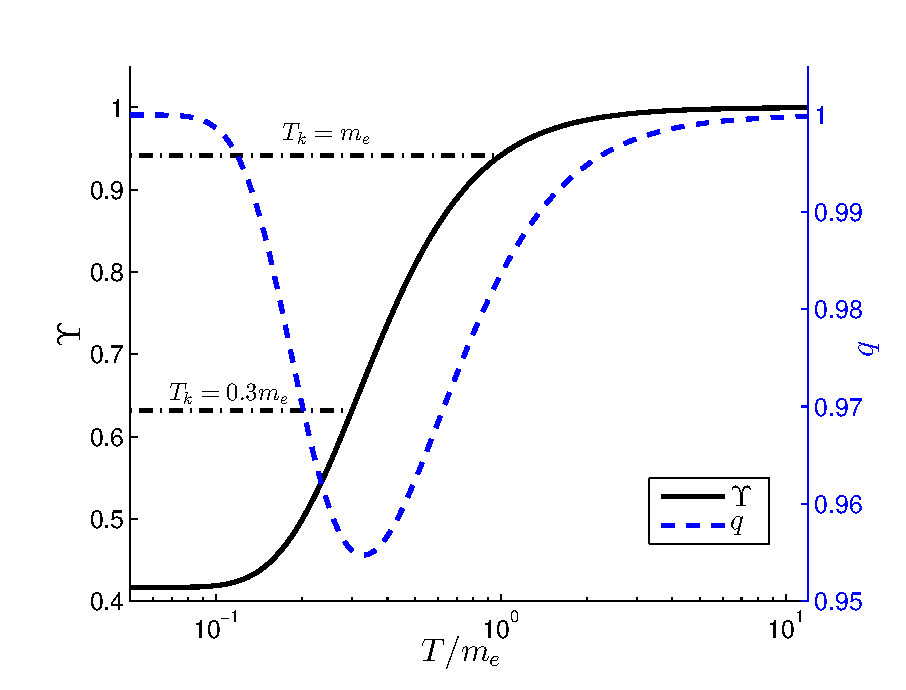
\includegraphics[height=5.8cm]{03-birrell/ModelIndStudy/Upsilon_q.eps}}
\makebox[0.5\linewidth]%
{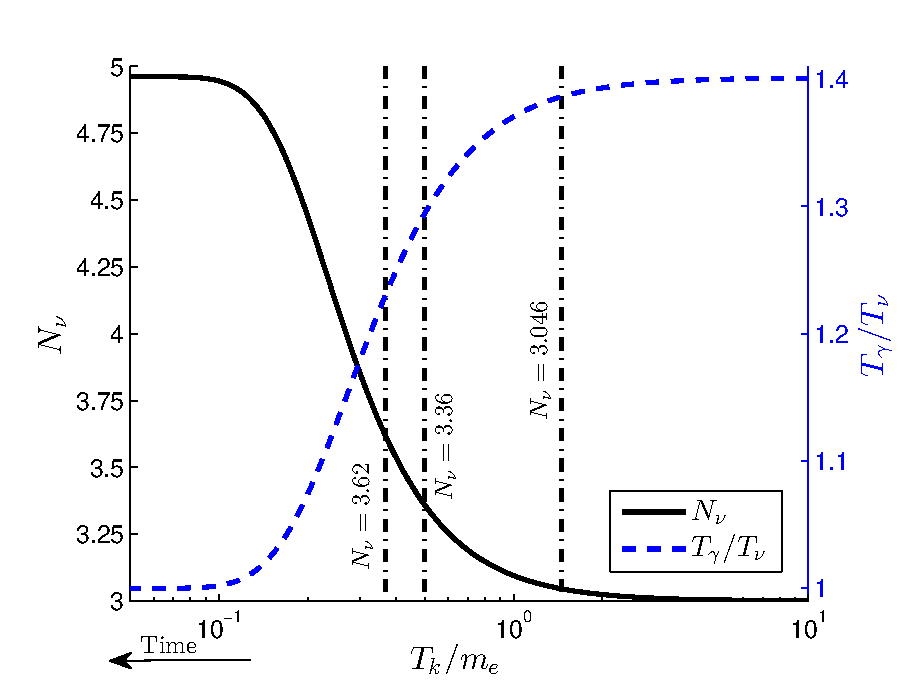
\includegraphics[height=5.8cm]{03-birrell/ModelIndStudy/N_eff.eps}}
\caption{Dependence of neutrino fugacity (left) and effective number of neutrinos and reheating ratio (right) on the neutrino kinetic freeze-out temperature. We also show the evolution of the deceleration parameter through the freeze-out period (left).}
\end{minipage}
 \end{figure}
%%%%%%%%%%%%%%%%%%%%%%%%%%%%%%%%%%%%%%%


These two papers also contain several figures that show other relations relation between the quantities $T_k$, $N_\nu$, $\Upsilon$, and $T_\gamma/T_\nu$ for which we do not have simple analytic relations. In figure \ref{fig:Tk_dependence} we give slightly modified versions of two of these plots, showing the dependence of $N_\nu$, $\Upsilon$, and $T_\gamma/T_\nu$ on $T_k$.  In particular, the fugacity evolves following the solid black curve in the left hand plot until it reaches the kinetic freeze-out temperature, at which point the neutrinos decouple and $\Upsilon$ remains constant thereafter, as shown in the dashed black curves for two sample values of $T_k$.

We showed in \cite{Birrell:2013_2} that after kinetic freeze-out, the free-streaming neutrino momentum distribution takes the form
\begin{equation}\label{neutrino_dist}
f(t,E)=\frac{1}{\Upsilon^{-1}e^{p/T_\nu}+ 1}
\end{equation}
where the neutrino effective temperature is redshifted as the universe expands
\begin{equation}\label{Tneutrino_dist}
T_\nu(t)\propto \frac{1}{a(t)}
\end{equation}
and the value of the fugacity  that developed during the freeze-out process is frozen into the distribution and remains constant while free-streaming. The resulting expressions for the energy density, pressure, and number density in the rest frame of the neutrino background are
\begin{align}
\rho&=\frac{g_\nu}{2\pi^2}\!\int_0^\infty\!\!\frac{\left(m_\nu^2+p^2\right)^{1/2}p^2dp }{\Upsilon^{-1}e^{p/T_\nu}+ 1},\label{neutrino_rho}\\[0.2cm]
P&=\frac{g_\nu}{6\pi^2}\!\int_0^\infty\!\!\frac{\left(m_\nu^2+p^2\right)^{-1/2}p^4dp }{\Upsilon^{-1} e^{p/T_\nu}+ 1},\label{neutrino_P}\\[0.2cm]
n&=\frac{g_\nu}{2\pi^2}\!\int_0^\infty\!\!\!\frac{p^2dp }{\Upsilon^{-1}e^{p/T_\nu}+ 1}.
\label{num_density}
\end{align}

  Finally, in  \cite{Birrell:2013_2} we presented for the first time a  physically consistent derivation of the equation of state of free-streaming neutrinos, including dependence on both $N_\nu$ and neutrino mass ($\beta=m_\nu/T_\gamma$). 
\begin{align}
&\rho^{EV}/\rho_0= N_\nu+0.1016\sum_i\beta_i^2+0.0015\delta N_\nu\sum_i\beta_i^2\notag\\
&-0.0001\delta N_\nu^2\sum_i\beta_i^2-0.0022\sum_i\beta_i^4,\\
&P^{EV}/P_0= N_\nu-0.0616\sum_i\beta_i^2-0.0049\delta N_\nu\sum_i\beta_i^2\notag\\
&+0.0005\delta N_\nu^2\sum_i\beta_i^2+0.0022\sum_i\beta_i^4.\label{tau_Ups}
\end{align}
The inclusion of fugacity was a crucial aspect in obtaining a physically consistent description, as it was in all of the above results.
